\chapter{Quantum Chromodynamics}
\label{chap:QCD}

The strong interaction is the fundamental force responsible for binding quarks together into hadrons. It is described by \ac{QCD} which is a gauge theory based on $SU(3)_{C}$ symmetry. One of the key features of \ac{QCD} is the phenomenon known as asymptotic freedom, namely strong force weakens at shorter distance. This property differentiates the strong force with all three other fundamental forces. A brief description of the formulation of \ac{QCD} is given in \autoref{sec:QCD}. Asymptotic freedom predicts that the strong coupling constant, denoted by $\alpha_{S}$, is small at short distance, which allows for perturbative expansion of the probability amplitude. However, the expansion parameter $\alpha_{S}$ at long distance becomes too large and the predictions are therefore no longer reliable. Techniques developed to model \ac{QCD} phenomenon in this regime are collectively known as nonperturbative-\ac{QCD}, which is discussed in \autoref{sec:Collision}.

\section{Formulation of QCD}
\label{sec:QCD}

The theory of strong interaction began taking its current form in 1964 when the quark model was independently proposed by American physicists George Zweig~\cite{Zweig:1964ruk} and his Ph.D. advisor Murray Gell-Mann~\cite{Gell-Mann:1964ewy}. The original objective of this model was to explain the spectrum of new hadrons discovered at rapid speed at the time. In this early version, mesons and baryons were viewed as composite objects formed by spin-$\frac{1}{2}$ particles, named ``quarks'' by Gell-Mann and ``aces'' by Zweig. They came with several quantum charges and three different flavors: $u$, $d$, $s$. The strange quarks in this model had a higher mass, which explained the mass differences between different baryons and mesons.

This model was successful in explaining why protons of same charge were bound together -- they were bound states of more fundamental particles affected by the strong interactions. However, gaps still existed in this model, mostly notably the tension with Fermi-Dirac statistics. It was indicated by this model that the wave function for $\mathrm{\Omega^{-}}$ (sss) should be symmetrical in the interchange of strange quarks. However, the wave function must be antisymmetric because quarks had half spins in this model. Gell-Mann and his collaborations was able resolve this problem in early 1970s by introducing color charges~\cite{Fritzsch:1973pi}. Under this updated framework, each flavor of quark should come with three colors, namely red, green, and blue. The wave functions of hadrons were assumed to be singlets of the gauge group $SU(3)_{C}$. For example, the wave function for $\mathrm{\Omega^{-}}$ baryon can be represented as,

\begin{equation}
(sss)\rightarrow(s_{r}s_{g}s_{b}-s_{g}s_{r}s_{b}+s_{b}s_{r}s_{g}-s_{r}s_{b}s_{g}+s_{g}s_{b}s_{r}-s_{b}s_{g}s_{r}),
\end{equation}

which restored the Fermi-Dirac statistics.  

The force mediators in this theory, known as ``gluons'', are massless vector bosons analogous to photons. They are electrically neutral but carry color charges, which enables the gluon-gluon self-interactions. The dynamics of gluon-gluon and quark-gluon interactions are described by the \ac{QCD} Lagrangian in the following form:

\begin{equation}
\mathcal{L}_{QCD}=-\frac{1}{2}\textsf{tr}G_{\mu\nu}G^{\mu\nu}+\bar{Q}(i\gamma^{\mu}D_{\mu}-m)Q,
\end{equation}

where $Q$ represents colour triplets quark fields $(Q_{r},Q_{g},Q_{b})^{T}$ of the $SU(3)_{C}$ group that run over six different flavors, $m$ corresponds to the mass of quarks. $G_{\mu\nu}$ is known as the gluon field strength tensor given by

\begin{equation}
\label{eq:G}
G_{\mu\nu}^{a}=\partial_{\mu}A_{\nu}^{a}-\partial_{\nu}A_{\mu}^{a}+g_{S}f^{abc}A_{\mu}^{b}A_{\nu}^{c},
\end{equation}

where $g_{S}$ corresponds to the strength of the gauge coupling. The strong coupling constant is also defined as $\alpha_{S}=\frac{g_{S}^2}{4\pi}$, which is analogous to the fine structure constant in \ac{QED}. $t_{a}$ are eight generators of the $SU(3)_{C}$ group, and $A^{a}_{\mu}$ represent eight gauge fields correspond to eight gluons. $f^{abc}$ is the structure constant defined by $[t^{a},t^{b}]=if^{abc}t^{c}$. $D_{\mu}$ is the $SU(3)_{C}$ gauge covariant derivative expresses as:

\begin{equation}
D_{\mu}=\partial_{\mu}-ig_{S}t_{a}A^{a}_{\mu}.
\end{equation}

The non-abelian structure of the $SU(3)_{C}$ group implies that the third term in Equation~\ref{eq:G} is nonzero as  $SU(3)_{C}$ generators do not commute with each other. This leads to the trilinear and quartic gluon self-interactions when expanding the kinetic (first) term of the QCD Lagrangian. 

In parallel to the development of the quark model, Feynman proposed a model to explain the behavior of hadron collisions~\cite{Feynman:1969wa}. Feynman postulated that protons are made of point-like constituents called ``partons'', and they behave like free particles at high momentum transfer, or equivalently short distance. The parton model was an immediate success as it was able to predict the short distance ``scaling'' effects of the strong interaction at a very good precision~\cite{Bjorken:1969ja}. Despite the success at describing experimental data, the parton model was still viewed as a phenomenological approximation as Feynman provided no microscopic description of the strong interactions. It was later understood that partons were matched to a collection of quarks and gluons within the nucleons.

Two years after Dutch physicist Gerard 't Hooft showed that non-abelian gauge theories were renormalizable~\cite{tHooft:1971akt}, major breakthrough came in 1973 when American physicists H. D. Politzer, David Gross, and Frank Wilczek~\cite{Gross:1973id,Politzer:1973fx} investigated the scale dependency of the strong coupling const $\alpha_{S}$. 't Hooft also arrived at similar results himself sometime earlier but he didn't publish his work. At one-loop precision, the $\alpha_{S}(\mu^2)$ is given by:

\begin{equation}
\label{eq:af}
\alpha_{S}(\mu^2)=\frac{\alpha_{S}(\mu_{R}^2)}{1+\beta_{0}\alpha_{S}(\mu_{R}^2)\textsf{ln}(\frac{\mu^2}{\mu_{R}^2})}
\end{equation}

where $\mu$ is the energy scale, $\mu_{R}$ is known as the renormalization scale, which corresponds to the energy initial scale at which $\alpha_{S}$ is evaluated. $\beta_{0}=(33-2n_{f})/12\pi$ is a constant that depends on the number quark flavors that can be considered massless. 

Equation~\ref{eq:af} reveals that when $n_{f}~<16$, the strength of the strong coupling decreases as energy increases. In other words, quarks and gluons behave like free particles at very short distance. The discovery of this property, known as ``asymptotic freedom'', by Politzer, Gross, and Wilczek brought the \ac{SM} to its current formulation. Since then it has withstood the test of numerous measurements of conducted at various experiments across a wide range of energy spectrum. A summary of recent measurements of $\alpha_{S}$ is given in Figure~\ref{fig:alphaS}.

\begin{figure}[tbh!]
 \begin{center}
 \begin{tabular}{c}
 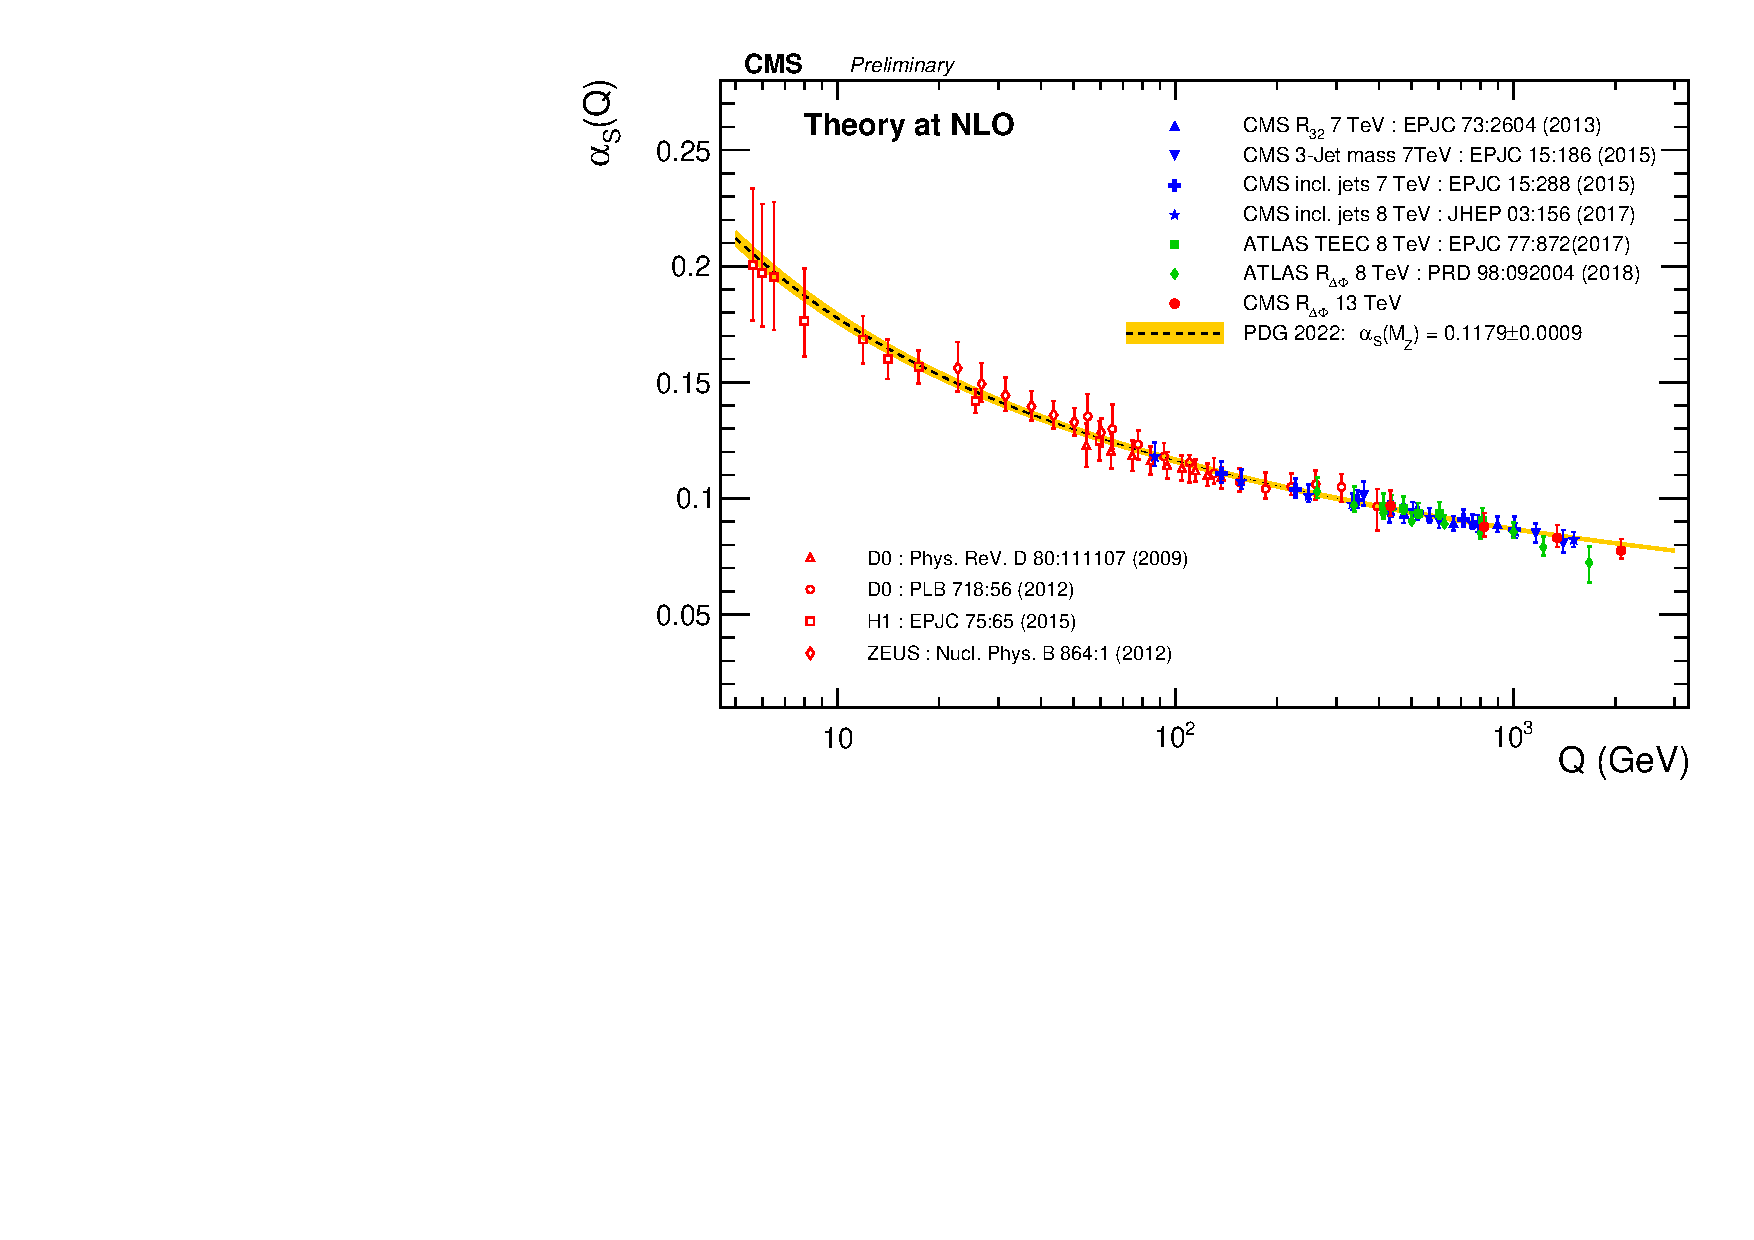
\includegraphics[width=0.8\textwidth]{figures/Part1/QCD/alphaS}
 \end{tabular}
 \caption{Summary of the running of $\alpha_{S}$ measured by \ac{CMS}, \ac{ATLAS} and other experiments. \cite{cms:twiki}}
 \label{fig:alphaS}
 \end{center}
\end{figure}

\section{Nonperturbative QCD and Hadron Collisions}
\label{sec:Collision}